% This is "sig-alternate.tex" V2.0 May 2012
% This file should be compiled with V2.5 of "sig-alternate.cls" May 2012
%
% This example file demonstrates the use of the 'sig-alternate.cls'
% V2.5 LaTeX2e document class file. It is for those submitting
% articles to ACM Conference Proceedings WHO DO NOT WISH TO
% STRICTLY ADHERE TO THE SIGS (PUBS-BOARD-ENDORSED) STYLE.
% The 'sig-alternate.cls' file will produce a similar-looking,
% albeit, 'tighter' paper resulting in, invariably, fewer pages.
%
% ----------------------------------------------------------------------------------------------------------------
% This .tex file (and associated .cls V2.5) produces:
%       1) The Permission Statement
%       2) The Conference (location) Info information
%       3) The Copyright Line with ACM data
%       4) NO page numbers
%
% as against the acm_proc_article-sp.cls file which
% DOES NOT produce 1) thru' 3) above.
%
% Using 'sig-alternate.cls' you have control, however, from within
% the source .tex file, over both the CopyrightYear
% (defaulted to 200X) and the ACM Copyright Data
% (defaulted to X-XXXXX-XX-X/XX/XX).
% e.g.
% \CopyrightYear{2007} will cause 2007 to appear in the copyright line.
% \crdata{0-12345-67-8/90/12} will cause 0-12345-67-8/90/12 to appear in the copyright line.
%
% ---------------------------------------------------------------------------------------------------------------
% This .tex source is an example which *does* use
% the .bib file (from which the .bbl file % is produced).
% REMEMBER HOWEVER: After having produced the .bbl file,
% and prior to final submission, you *NEED* to 'insert'
% your .bbl file into your source .tex file so as to provide
% ONE 'self-contained' source file.
%
% ================= IF YOU HAVE QUESTIONS =======================
% Questions regarding the SIGS styles, SIGS policies and
% procedures, Conferences etc. should be sent to
% Adrienne Griscti (griscti@acm.org)
%
% Technical questions _only_ to
% Gerald Murray (murray@hq.acm.org)
% ===============================================================
%
% For tracking purposes - this is V2.0 - May 2012

\documentclass{sig-alternate}

\begin{document}

\title{Searching Web Data using MinHash LSH}
%
% You need the command \numberofauthors to handle the 'placement
% and alignment' of the authors beneath the title.
%
% For aesthetic reasons, we recommend 'three authors at a time'
% i.e. three 'name/affiliation blocks' be placed beneath the title.
%
% NOTE: You are NOT restricted in how many 'rows' of
% "name/affiliations" may appear. We just ask that you restrict
% the number of 'columns' to three.
%
% Because of the available 'opening page real-estate'
% we ask you to refrain from putting more than six authors
% (two rows with three columns) beneath the article title.
% More than six makes the first-page appear very cluttered indeed.
%
% Use the \alignauthor commands to handle the names
% and affiliations for an 'aesthetic maximum' of six authors.
% Add names, affiliations, addresses for
% the seventh etc. author(s) as the argument for the
% \additionalauthors command.
% These 'additional authors' will be output/set for you
% without further effort on your part as the last section in
% the body of your article BEFORE References or any Appendices.

\numberofauthors{2} %  in this sample file, there are a *total*
% of EIGHT authors. SIX appear on the 'first-page' (for formatting
% reasons) and the remaining two appear in the \additionalauthors section.
%
\author{
% You can go ahead and credit any number of authors here,
% e.g. one 'row of three' or two rows (consisting of one row of three
% and a second row of one, two or three).
%
% The command \alignauthor (no curly braces needed) should
% precede each author name, affiliation/snail-mail address and
% e-mail address. Additionally, tag each line of
% affiliation/address with \affaddr, and tag the
% e-mail address with \email.
%
% 1st. author
\alignauthor
BiChen Rao\\
       \affaddr{University of Toronto}\\
       \email{eric.rao@mail.utoronto.ca}
% 2nd. author
\alignauthor
Erkang Zhu\\
       \affaddr{University of Toronto}\\
       \email{ekzhu@cs.toronto.edu}
}
% There's nothing stopping you putting the seventh, eighth, etc.
% author on the opening page (as the 'third row') but we ask,
% for aesthetic reasons that you place these 'additional authors'
% in the \additional authors block, viz.

\maketitle
\begin{abstract}
In this extended abstract, we explore the use of MinHash Locality Sensitive Hashing
(MinHash LSH) to address the problem of indexing and searching Web data.
We discuss a statistical tuning strategy for MinHash LSH index, and
experimentally evaluate the accuracy and performance of MinHash LSH, with comparison against inverted index.
In addition, we describe an on-line demo for the 
index with real Web data.
\end{abstract}

\section{Introduction}
Numerous datasets are published on the Web and can be used freely.
The Web Data Common Web Table project extracted over 200 millions tabular 
datasets from HTML pages on the Web~\cite{Lehmberg:WWW:2016}.
With the huge amount of data available, it is difficult for researchers to discover datasets covering similar topics, due to their heterogeneous sources and schemas and the lack of search infrastructure. Datasets can be huge in size and the number of datasets is usually massive, causing additional challenges to Web data search.

When searching for attributes, we can use the Jaccard distance between
{\it attributes} of the datasets as relevance measure.
An attribute is a set of values. 
It can be extracted from a column of a tabular dataset, or a full path in
a semi-structured dataset.
Due to the massive scale in the size and number of attributes,
computing Jaccard distance directly using data values can be very expensive.
We can represent an attribute with a fixed-size summary called {\it MinHash},
which consist of a set of hash values from a group of minwise hash functions in order to reduce the storage size and increase the query/insertion speed~\cite{Broder:1997:RCD:829502.830043}.
However, with over millions of attributes, linear scan over MinHashes is still very slow.
MinHash LSH can be used to index the MinHashes of attributes~\cite{Indyk:1998:ANN:276698.276876}. 
Similar attributes can be searched by querying a number of hash tables whose hash keys are concatenations of hash values in MinHash, in sub-linear time with respect to the number of attributes.
SimHash is an alternative LSH index that also support sub-linear search time~\cite{Charikar:2002:SET:509907.509965}, however,
a recent paper showed that MinHash LSH is more computationally efficient than SimHash~\cite{simhash:minhash}.

In this extended abstract, we present our work on indexing and searching
attributes using MinHash LSH, and experimental evaluation with real Web data.

\section{Tuning MinHash LSH}
Minhash LSH has two parameters: $L$ the number of hash tables
and $M$ the size of the hash key, which is a concatenation of 
$M$ hash values in MinHash.
The parameters typically need to be hand-tuned for balancing
accuracy and performance.

We used a statistical tuning strategy based on the one proposed by Dong et al. 
for Euclidean distance~\cite{Dong:2008:MLP:1458082.1458172}.
The following distributions need to be obtained from the data: 
(1) the distribution of all-pair squared Jaccard distance, and
(2) given $K$, the distribution of squared Jaccard distance for the
$1^{st}$ to $K^{th}$ ranked attributes.
The tuning is formulated as an optimization problem, where the objective
is to minimize {\it selectivity}, which is defined as the number of matches 
returned by LSH divided by the total number of attributes in the index, while 
maintaining a minimum level of {\it recall}. 
In other words, we want to minimize the processing cost for the returned matches
without loosing too much accuracy. 
The selectivity can be expressed as:
\begin{equation}
selectivity = \int_{0}^{1.0} \rho(\sqrt{x})f(x)dx\\
\end{equation}
And the recall can be expressed as:\\
\begin{equation}
recall = \frac{1}{K} \sum_{k=1}^{K} \int_{0}^{1.0} \rho(\sqrt{x})f_k(x)dx\\
\end{equation}
$f(.)$ is the squared Jaccard distance distribution of all-pairs and $f_k(.)$ is the squared Jaccard distance distribution of the $K$th result. 
$\rho(.)$ is the probability of LSH returning the result given the distance to the 
the query data.
$\rho(.)$ can be obtained using a closed form equation given $M$ and $L$.\cite{rp:close}.

\section{Experimental Evaluation}
To evaluate the accuracy and performance of MinHash LSH index, we downloaded the English Relation subset of the 2015 Web Data Common Web Table~\cite{Lehmberg:WWW:2016}.
It contains 51 million tables and 262,893,349 attributes (i.e. columns) in total.

\noindent {\bf Accuracy}
We take a random sample of 1,000 tables
to estimate the distributions required for index tuning. 
The all-pair square Jaccard distance distribution is plotted on left side of Figure~\ref{fig:jsim}. The right side of Figure~\ref{fig:jsim} shows the squared Jaccard distance distributions for the $10^{th}$, $20^{th}$, $50^{th}$ ranked in the top-$K$ matches. 
We fit the distributions with gamma functions, and use the fitted gamma functions to approximate the probability density functions of the original distributions.
For index tuning, we choose the minimum recall to be 0.6.
The optimal parameters are $M = 2$ and $L = 256$.
We build the index using 1,000 random selected tables.
Table~\ref{table:rfp} presents the average precision and recall of 1,000 randomly selected
query attributes. We can see the recalls are very close to the minimum recall
set in index tuning.

\begin{figure}[t]
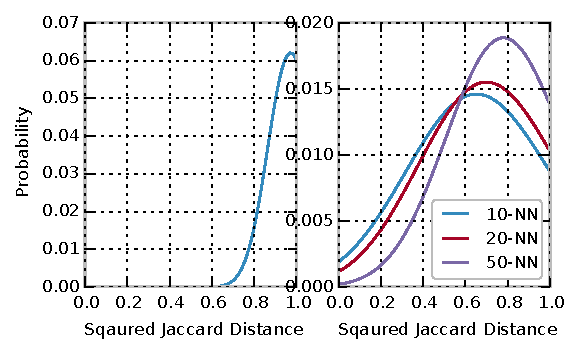
\includegraphics[width=\columnwidth, natwidth=1, natheight=1]{dist_dist.pdf}
\caption{Squared Jaccard Distance Distribution for Attributes in Web Table}
\label{fig:jsim}
\end{figure}

\begin{table}
\begin{tabular}{|c|c|c|c|} \hline
K&Precision&Recall&F Score\\ \hline
10&0.716&0.584&0.643\\\hline
30&0.738&0.564&0.639\\\hline
50&0.775&0.583&0.665\\\hline

\end{tabular}
\centering
\caption{Precision, Recall and F-score for different $K$s}
\label{table:rfp}
\end{table}


\noindent {\bf Performance}
An alternative search index is inverted index. In our experiment, the inverted index is constructed by building a mapping from data value to attributes. For query, MinHash LSH has a time complexity of $O(L\cdot M)$ since it only needs to query $L$ hash tables to retrieve the appropriate attributes, and each hash key is a concatenation of $M$ hash values. The inverted index has a time complexity of $O(log(N)\cdot q)$ where $N$ is the number of indexed attributes and $q$ is the number of distinct data values in the query attribute,
since for each data value, the index finds all attributes that contain it.
Figure \ref{fig:lsh_inverted} shows the query time of inverted index vs. MinHash LSH with respect to increasing number of indexed attributes. The query time of the MinHash LSH index stays constant, while the query time of the inverted index increases in a logarithmic fashion. Thus, the result confirms the previous analysis.

\begin{figure}[t]
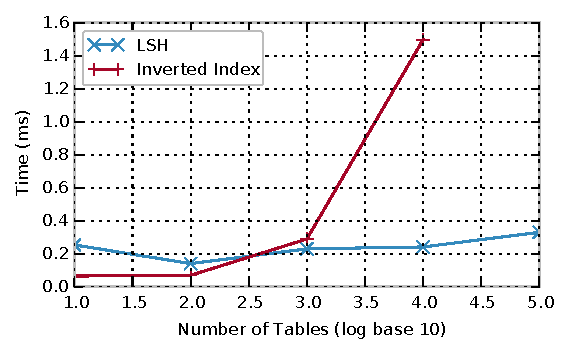
\includegraphics[width=\columnwidth, natwidth=1, natheight=1]{lsh_time.pdf}
\caption{MinHash LSH vs Inverted Index Performance}
\label{fig:lsh_inverted}
\end{figure}

% \section{Implementation}
% \noindent {\bf Data Storage}
% A data storage is necessary for the LSH index to retrieve the relevant signatures using the result keys. Since no statistical analysis will be performed on the store value, a NoSQL Database such as redis, Cassendra or HBase is best suited for the task. The Redis database has the lowest read latency with a reasonable throughput and scalability according to \cite{redis:compare}.\\
% {\bf Web Framework} For the demonstration application we choose the ReST frame work for the generality of its interfaces.\cite{Fielding:2000:ASD:932295}\\
% {\bf Programming language}
% The query process of the LSH index are parallelizable to increase the throughput of the application. Several bench mark tests have shown that the programming language Go achieve better parallelism than python in most of the test cases with go routine. \cite{go:benchmark}

\section{Demo}
A demo of the MinHash LSH index with Web Table data can be accessed at
{\tt vldb.cs.toronto.edu:4001}.
A user can upload a CSV file to the website and retrieve tables that contain similar columns as the input CSV file.
The demo application uses a MinHash LSH index with
10 million indexed tables.
Redis, a distributed key-value store, is used to implement the MinHash LSH index.
Using Redis allows the index to scale beyond a single machine and support high
throughput.

\section{Conclusion and Future Work}
We have shown that MinHash LSH is very efficient for searching datasets,
and a statistical tuning strategy can be used to balance the performance 
and recall accuracy.
Alternative LSH indexes such as LSH Forest~\cite{Bawa:WWW:2005} can be used to further improve
accuracy.
Furthermore, set containment is often a better measure of relevance than 
Jaccard distance. Using LSH for set containment search is another 
direction of research.
%
% The following two commands are all you need in the
% initial runs of your .tex file to
% produce the bibliography for the citations in your paper.
\bibliographystyle{plain}
\bibliography{paper}  % sigproc.bib is the name of the Bibliography in this case
% You must have a proper ".bib" file
%  and remember to run:
% latex bibtex latex latex
% to resolve all references
%
% ACM needs 'a single self-contained file'!
%
\end{document}
